\documentclass{article}

\usepackage{graphicx}
\usepackage{tikz}
\usepackage{tikzsymbols}
\usetikzlibrary{calc,patterns,shapes.geometric}
\pagestyle{empty}
\usepackage[margin=0pt]{geometry}
\geometry{papersize={14in,12in}}

\def\centerarc[#1](#2)(#3:#4:#5){\draw[#1] ($(#2)+({#5*cos(#3)},{#5*sin(#3)})$) arc (#3:#4:#5);}

\begin{document}
	\begin{figure}
		\centering
		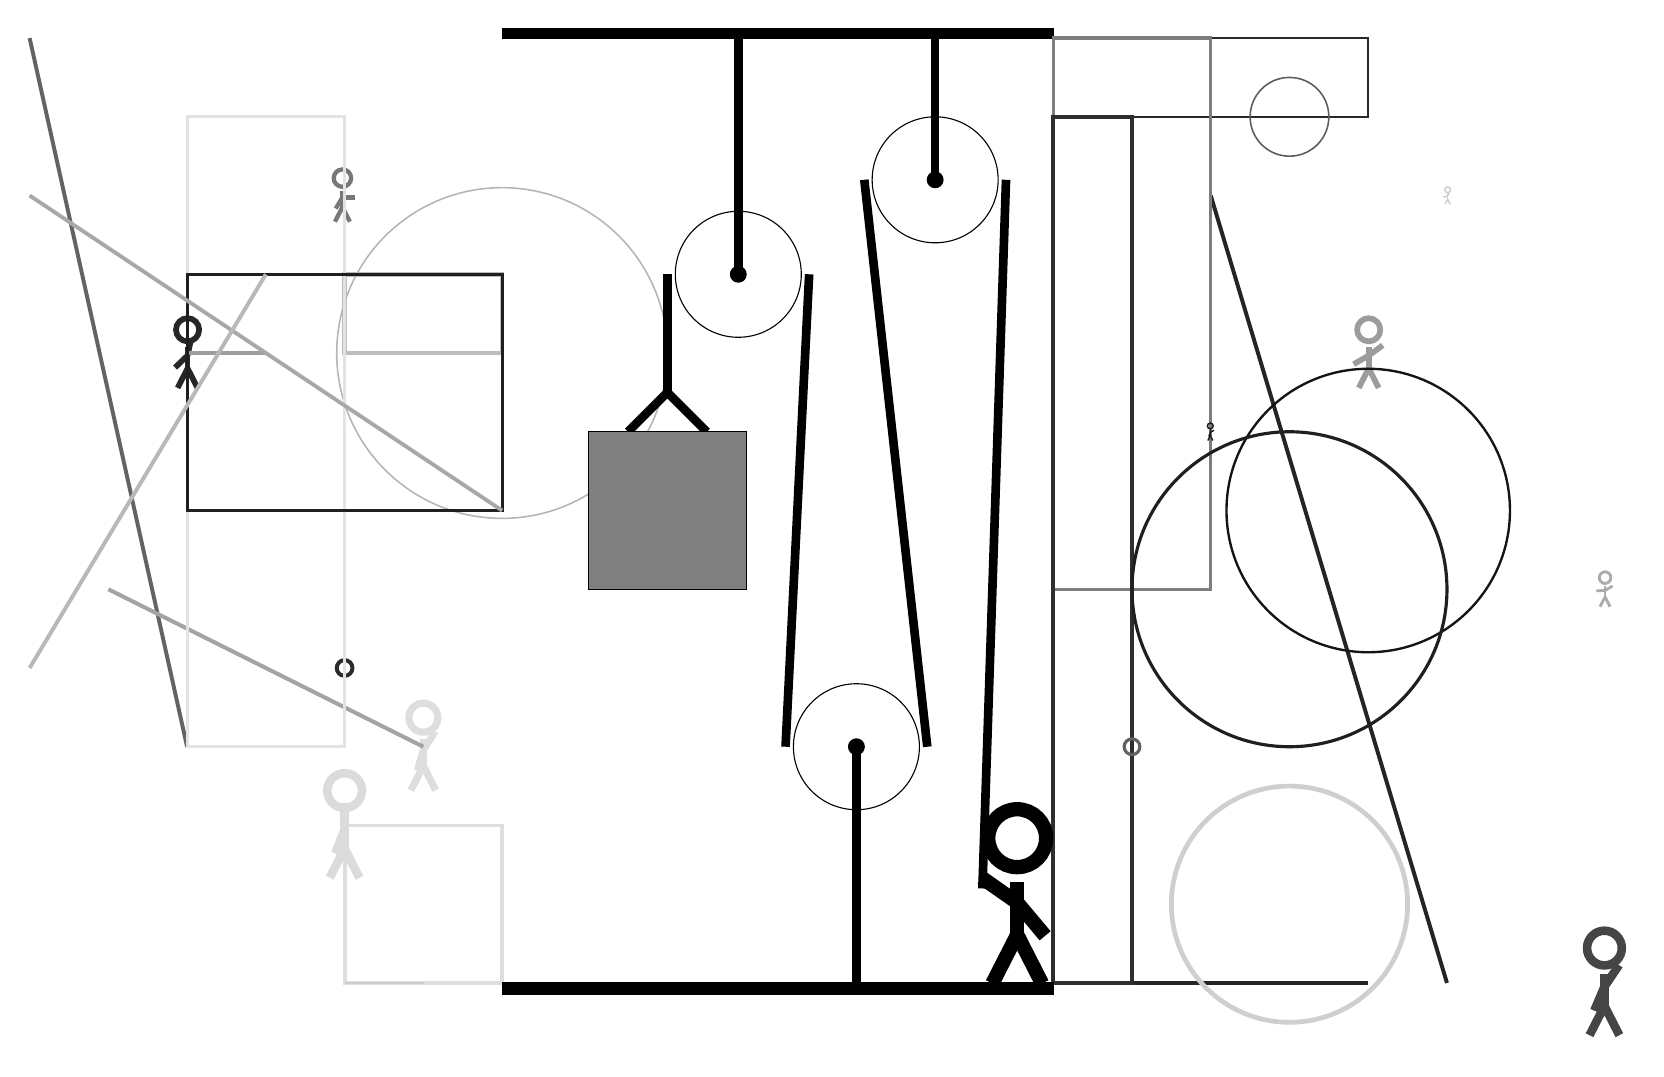
\begin{tikzpicture}
			%%%%% START %%%%%
			
			\draw[fill=black] (-2, 9) rectangle (5, 9.125);
			
			\draw (1, 6) circle (0.8);
			\draw[fill=black] (1, 6) circle (0.1);
			\draw[line width=1.1mm]  (1, 9) -- (1, 6);
			
			\draw[fill=white](2.5, 0) circle (0.8);
			\draw[fill=black] (2.5, 0) circle (0.1);
			\draw[line width=1.1mm]  (2.5, -3) -- (2.5, 0);
			
			\draw[fill=white](3.5, 7.2) circle (0.8);
			\draw[fill=black] (3.5, 7.2) circle (0.1);
			\draw[line width=1.1mm] (3.5, 9) -- (3.5, 7.2);
			
			\draw[line width=0.5mm, color=black!86](7, 7) -- (10, -3);
			
			\node[line width=0.2mm, color=black!39] at (9, 5) {\Strichmaxerl[4][30][36]};
			\node[line width=0.2mm, color=black!33] at (12, 2) {\Strichmaxerl[2][2][31]};
			\node[line width=0.5mm, color=black!85] at (-6, 5) {\Strichmaxerl[4][44][78]};
			\draw[line width=0.3mm, color=black!84] (5, 8) rectangle (9, 9);
			
			\draw[line width=0.6mm, color=black!26] (-4, 6) rectangle (-2, 5);
			\node[line width=0.3mm, color=black!53] at (-4, 7) {\Strichmaxerl[3][59][0]};
			
			\draw [line width=0.5mm, color=black!83](-4, 1) circle (0.1);
			\node[line width=0.4mm, color=black!13] at (-3, 0) {\Strichmaxerl[5][74][57]};
			\draw[line width=0.5mm, color=black!13] (-2, -3) rectangle (-4, -1);
			
			\draw [line width=0.2mm, color=black!29](-2, 5) circle (2.1);
			\node[line width=0.2mm, color=black!20] at (10, 7) {\Strichmaxerl[1][11][72]};
			\draw[line width=0.5mm, color=black!61](-6, 0) -- (-8, 9);
			\draw[line width=0.4mm, color=black!51] (5, 9) rectangle (7, 2);
			\node[line width=0.7mm, color=black!14] at (-4, -1) {\Strichmaxerl[6][69][90]};
			\draw[line width=0.5mm, color=black!36](-3, 0) -- (-7, 2);
			
			\draw[line width=0.4mm, color=black!11] (-4, 0) rectangle (-6, 8);
			
			\draw[line width=0.2mm, color=black!20] (-4, -3) rectangle (-3, -3);
			\draw[line width=0.5mm, color=black!38](-6, 5) -- (-5, 5);
			\draw[line width=0.5mm, color=black!86](9, -3) -- (6, -3);
			\draw [line width=0.2mm, color=black!64](8, 8) circle (0.5);
			\node[line width=0.3mm, color=black!73] at (12, -3) {\Strichmaxerl[6][67][56]};
			\draw[line width=0.4mm, color=black!88] (-2, 3) rectangle (-6, 6);
			\draw [line width=0.6mm, color=black!19](8, -2) circle (1.5);
			\node[line width=0.7mm, color=black!90] at (7, 4) {\Strichmaxerl[1][70][30]};
			\draw[line width=0.5mm, color=black!82] (5, 8) rectangle (6, -3);
			\draw[line width=0.5mm, color=black!34](-2, 3) -- (-8, 7);
			\draw [line width=0.3mm, color=black!92](9, 3) circle (1.8);
			\draw [line width=0.4mm, color=black!88](8, 2) circle (2.0);
			\draw [line width=0.4mm, color=black!61](6, 0) circle (0.1);
			\draw[line width=0.5mm, color=black!28](-5, 6) -- (-8, 1);
			
			\draw[line width=1.1mm] (-0.4, 4.0) -- (0.1, 4.5) -- (0.6, 4.0);
			\draw[fill=black!50] (-0.9, 4.0) rectangle (1.1, 2.0);
			
			\draw[line width=1.1mm] (0.1, 6) -- (0.1, 4.5);
			\centerarc[line width=1.1mm](1, 6)(0:180:0.9);
			\draw[line width=1.1mm](1.9, 6) -- (1.6, 0);
			\centerarc[line width=1.1mm](2.5, 0)(180:360:0.9);
			\draw[line width=1.1mm](3.4, 0) -- (2.6, 7.2);
			\centerarc[line width=1.1mm](3.5, 7.2)(0:180:0.9);
			\draw[line width=1.1mm](4.4, 7.2) -- (4.1, -1.8);
			
			\node at (4.5, -1.9) {\Strichmaxerl[10][-35][-50]};
			
			\draw[fill=black] (-2, -3) rectangle (5, -3.15);
			
			%%%%% END %%%%%
		\end{tikzpicture}
	\end{figure}	
\end{document}